% xelatex </dev/null myricube25.tex
% This has nothing to do with spork/Exo-GPU but it's here anyway...
%
% Background: voxel rendering
%   Memory-intensive
%   Cubic growth in detail (without tricks)
%   Fast rendering - more upfront work
%   Fast loading & edits -- less upfront work
%   Real-world applications: OMG none
%
% Compute vs. graphics
%   Explicit vs implicit parallelism
%
% Vertex Shading
%
% Fragment Shading
%
% Voxels-to-triangles
%
% Raycasting
%
% Both: translate voxel grid to another format
%   Zero-in on data that matters
%   Skip work
%
% Magic of graphics pipeline
%
% Implicit sequential semantics
%
% Workload balancing
%
% Early z-culling
%
% Chunks: 16 × 16 × 16 voxels
%   AABB
%   Draw AABB (12 triangles), raycast only within chunk
%
% Demo 1
%
% Reverse Painters
%   Only waste 12 tringles, not thousands/millions
%
% Upload from disk
%
% Demo 2
\documentclass[12pt]{article}

\usepackage[paperheight=148mm, paperwidth=263mm, margin=10mm]{geometry}
\usepackage{enumitem}
\usepackage{amsmath}
\usepackage{amssymb}
\usepackage{amsfonts}
\usepackage{placeins}
\usepackage{graphicx}
\usepackage{listings}
\usepackage{caption}
\usepackage{colortbl}
\usepackage[parfill=0pt]{parskip}
\usepackage[mathscr]{euscript}
\usepackage[usenames,dvipsnames,svgnames,table,hyperref]{xcolor}
\usepackage[hidelinks]{hyperref}
\usepackage{fontspec}
\usepackage{mdframed}
\usepackage{tikz}
\usetikzlibrary{shapes.geometric, arrows, positioning, calc}

\setsansfont{FreeSans}
\setmonofont{Ubuntu Mono}
\renewcommand{\familydefault}{\sfdefault}

\hyphenation{WebGL}

\definecolor{webColor}{RGB}{0, 108, 174}
\newcommand{\web}[1]{{\color{webColor} \small \url{#1}}}
\newcommand{\webText}[2]{{\color{webColor} \href{#2}{#1}}}
\newcommand{\email}[2]{{\small \color{webColor} \textsf{\href{mailto:#1@#2}{#1[at]#2}}}}
\definecolor{titleColor}{RGB}{179, 0, 149}
\definecolor{extraTitleColor}{RGB}{0, 149, 224}
\newcommand{\myTitle}[1]{{\large \color{titleColor} \hspace{-4mm} \textbf{\textsf{#1}}}}
\newcommand{\myTitleExtra}[1]{{\large \color{extraTitleColor} \hspace{-4mm} \textbf{\textsf{#1}}}}
\newcommand{\myBiggerTitle}[1]{{\huge \color{titleColor} \hspace{-4mm} \textbf{\textsf{#1}}}}
\newcommand{\myBiggerTitleExtra}[1]{{\huge \color{extraTitleColor} \hspace{-4mm} \textbf{\textsf{#1}}}}
\definecolor{subColor}{RGB}{179, 0, 149}
\newcommand{\mySub}[1]{\textsf{\color{subColor}$\blacktriangleright$ #1}}
\definecolor{keyColor}{RGB}{170, 149, 0}  % legacy, = keyColorA
\definecolor{keyColorA}{RGB}{170, 149, 0}
\definecolor{keyColorB}{RGB}{170, 210, 0}
\newcommand{\myKey}[1]{\textbf{\color{keyColor}#1}}
\newcommand{\myKeyA}[1]{\textbf{\color{keyColor}#1}}
\newcommand{\myKeyB}[1]{\textbf{\color{keyColorB}#1}}

% Red and blue boxes have bright text color.
% Yellow, green, and violet have intentionally muted text colors.
% They used to be black, but it looks slightly better with a tiny bit of color.
\definecolor{redBoxFg}{RGB}{224, 0, 0}
\definecolor{redBoxBg}{RGB}{255, 211, 225}
\newcommand{\redBox}[1]{{\color{redBoxFg}\colorbox{redBoxBg}{#1}}}
\definecolor{yellowBoxFg}{RGB}{89, 89, 0}
\definecolor{yellowBoxBg}{RGB}{255, 232, 0}
\newcommand{\yellowBox}[1]{{\color{yellowBoxFg}\colorbox{yellowBoxBg}{#1}}}
\definecolor{greenBoxFg}{RGB}{0, 89, 63}
\definecolor{greenBoxBg}{RGB}{179, 232, 160}
\newcommand{\greenBox}[1]{{\color{greenBoxFg}\colorbox{greenBoxBg}{#1}}}
\definecolor{blueBoxFg}{RGB}{0, 97, 232}
\definecolor{blueBoxBg}{RGB}{224, 232, 255}
\newcommand{\blueBox}[1]{{\color{blueBoxFg}\colorbox{blueBoxBg}{#1}}}
\definecolor{violetBoxFg}{RGB}{108, 63, 124}
\definecolor{violetBoxBg}{RGB}{218, 204, 255}
\newcommand{\violetBox}[1]{{\color{violetBoxFg}\colorbox{violetBoxBg}{#1}}}

\mdfdefinestyle{MyFrame}{%
    linecolor=black,
    outerlinewidth=0pt,
    linewidth=0pt,
    innertopmargin=2.7pt,
    innerbottommargin=0pt,
    innerrightmargin=0pt,
    innerleftmargin=0pt,
        leftmargin = 0pt,
        rightmargin = 0pt}


\definecolor{lightttColor}{RGB}{69, 69, 80}
\newcommand{\lighttt}[1]{{\color{lightttColor}\texttt{#1}}}
\newcommand{\blacktt}[1]{{\color{black}\texttt{#1}}}
\definecolor{grayttColor}{RGB}{144, 144, 160}
\newcommand{\graytt}[1]{{\color{grayttColor}\texttt{#1}}}
\definecolor{emphttColor}{RGB}{170, 149, 0}
\newcommand{\emphtt}[1]{{\color{emphttColor}\texttt{#1}}}

\renewcommand*\labelenumi{(\theenumi)}
\renewcommand*{\theenumii}{\roman{enumii}}
\renewcommand*\labelenumii{\theenumii.}

\newcommand{\fixminipage}{\raggedright \setlength{\parskip}{0.3\baselineskip}}
\newcommand{\codeminipage}{\raggedright \setlength{\parskip}{0\baselineskip}}
\sloppy
%\pagenumbering{gobble}


\tikzstyle{arrow} = [thick,->,>=stealth]
\tikzstyle{line} = [thick]

\tikzstyle{basic} = [rectangle, minimum height=1cm, text centered, draw=black, fill=white, text=black]
\tikzstyle{redstyle} = [draw=redBoxFg, fill=redBoxBg, text=redBoxFg]
\tikzstyle{yellowstyle} = [draw=yellowBoxFg, fill=yellowBoxBg, text=yellowBoxFg]
\tikzstyle{greenstyle} = [draw=greenBoxFg, fill=greenBoxBg, text=greenBoxFg]
\tikzstyle{bluestyle} = [draw=blueBoxFg, fill=blueBoxBg, text=blueBoxFg]
\tikzstyle{violetstyle} = [draw=violetBoxFg, fill=violetBoxBg, text=violetBoxFg]
\tikzstyle{nRedstyle} = [draw=nRedBoxFg, fill=nRedBoxBg, text=nRedBoxFg]
\tikzstyle{nGoldstyle} = [draw=nGoldBoxFg, fill=nGoldBoxBg, text=nGoldBoxFg]
\tikzstyle{nGreenstyle} = [draw=nGreenBoxFg, fill=nGreenBoxBg, text=nGreenBoxFg]
\tikzstyle{nBluestyle} = [draw=nBlueBoxFg, fill=nBlueBoxBg, text=nBlueBoxFg]
\tikzstyle{nPurplestyle} = [draw=nPurpleBoxFg, fill=nPurpleBoxBg, text=nPurpleBoxFg]
\tikzstyle{cheesyvertex} = [text width=2mm, text height=2mm, anchor=center]

\begin{document}

\hfill\myBiggerTitle{Myricube: Adventures in Voxel Rendering \& Fast Edits}

\includegraphics[width=\linewidth]{myricube/title.jpg}

\newpage
\myBiggerTitle{Voxel Rendering Background}

{\LARGE

3D voxel grid $\to$ 2D color image

Voxel = int-aligned $1 \times 1 \times 1$ cube

\begin{itemize}
  \item Opaque color, or ``transparent'' (for my purposes)
\end{itemize}

Minecraft render distance is lame: why is it hard to scale?

\vfill

\includegraphics[width=\linewidth]{myricube/background_0.jpg}

}

\newpage
\myBiggerTitle{Voxel Rendering Scaling Challenges}

{\LARGE

Challenge: memory-intensive (cubic-ish in render distance)

Challenge: High \# of triangles, sharp detail (low pixels per voxel)

\vfill

\includegraphics[width=0.4\linewidth]{myricube/background_1.jpg}
\includegraphics[width=0.4\linewidth]{myricube/background_2.jpg}

}

\newpage
\myBiggerTitle{Voxel Rendering Goals}

{\LARGE
My goals: think Minecraft, not scientific visualization

\vspace{4mm}

\begin{enumerate}
  \item High render distance at full detail (no level-of-detail)
  \item Fast rendering (motivates \myKeyA{more} upfront work)
  \item Fast loading \& edits (motivates \myKeyA{less} upfront work)
\end{enumerate}

\vspace{4mm}

Real-world applications... OMG, NONE!

Ex post facto goal: learn Vulkan and convince Nvidia to hire me

}

\newpage
\myBiggerTitle{GPU: Compute vs Graphics API}

{\large
\begin{tikzpicture}[node distance=0mm]
\node (cpu) [basic, text width=42mm] {\textbf{CPU} API calls};
\node (compute) [basic, text width=42mm, anchor=north east, yshift=-4mm] at(cpu.south west) {\textbf{Compute API}\\e.g. CUDA};
\node (graphics) [basic, text width=42mm, anchor=north west, yshift=-4mm] at(cpu.south east) {\textbf{Graphics API}\\e.g. OpenGL};

\node (grids) [basic, text width=60mm, anchor=north, yshift=-4mm] at(compute.south) {\textbf{Verb:} launch grids\\ (\myKeyA{explicitly parallel})};
\node (triangles) [basic, text width=80mm, anchor=north, yshift=-4mm] at(graphics.south) {\textbf{Verb:} draw triangles / primitives\\ (\myKeyA{sequential semantics}, mostly)};

\node (gpu) [basic, thick, draw=nGreenBoxBg, text width=190mm, anchor=north, text height=26mm, yshift=-46mm] at(cpu.south) {};
\node (vertex) [basic, nPurplestyle, text width=55mm, anchor=north, yshift=-50mm] at(cpu.south) {Runs\\\textbf{Vertex Shaders}\\(positions each vertex)};
\node (fragment) [basic, greenstyle, text width=55mm, anchor=west, xshift=6mm] at(vertex.east) {Runs\\\textbf{Fragment Shaders}\\(colors interior pixels)};
\node (thread) [basic, text width=55mm, anchor=east, xshift=-6mm] at(vertex.west) {Runs\\\textbf{CUDA Threads}\\(grouped into CTAs)};
\node (gpuCaption) [text=nGreenBoxBg, anchor=north west] at(gpu.south west) {\textbf{Execution on programmable GPU}};

\draw [arrow] (cpu.south) to[out=270, in=0] (compute.east);
\draw [arrow] (cpu.south) to[out=270, in=180] (graphics.west);
\draw [line] (compute.south) -- (grids.north);
\draw [line] (graphics.south) -- (triangles.north);
\draw[arrow] (grids.south) to[out=270, in=90] (thread.north);
\draw[arrow] (triangles.south) to[out=270, in=90] (vertex.north);
\draw[arrow] (triangles.south) to[out=270, in=90] (fragment.north);

\node (v0) [yshift=-20mm, xshift=+3mm, fill=nPurpleBoxBg, cheesyvertex] at(vertex.south) {};
\node (v1) [yshift=-10mm, xshift=+43mm, fill=nPurpleBoxBg, cheesyvertex] at(vertex.south) {};
\node (v2) [yshift=-35mm, xshift=+30mm, fill=nPurpleBoxBg, cheesyvertex] at(vertex.south) {};
\fill [greenBoxBg] (v0.center) -- (v1.center) -- (v2.center) -- cycle;

\draw [arrow, dotted] (vertex) -- (v0);
\draw [arrow, dotted] (vertex) -- (v1);
\draw [arrow, dotted] (vertex) -- (v2);
\draw [arrow, dotted] (fragment.south) to[out=270, in=0] ($(v2)!0.5!(v1) + (-0.3,0)$);

\node (etc) [text width=80mm, yshift=-6mm, anchor=north west] at(gpuCaption.south west) {Not shown, GPU primitive gen:\\geometry, tess, mesh, task shaders};

\end{tikzpicture}
}
\newpage
\myBiggerTitle{Vertex Shading (Triangle Strip Topology)}

{\large
\begin{tikzpicture}[node distance=0mm]

\node (vb00) [basic, text width=10mm, text height=10mm, anchor=north] {};
\node (vb01) [basic, text width=10mm, text height=10mm, anchor=north] at(vb00.south) {};
\node (vb02) [basic, text width=10mm, text height=10mm, anchor=north] at(vb01.south) {};
\node (vb03) [basic, text width=10mm, text height=10mm, anchor=north] at(vb02.south) {};
\node (vb04) [basic, text width=10mm, text height=10mm, anchor=north] at(vb03.south) {};
% \node (vb05) [text centered, text width=10mm, anchor=north] at(vb04.south) {\Huge $\downarrow$\\$\downarrow$};

\node (text0) [anchor=east, text height=10mm] at(vb00.west) {Vertex 0};
\node (text1) [anchor=east, text height=10mm] at(vb01.west) {Vertex 1};
\node (text2) [anchor=east, text height=10mm] at(vb02.west) {Vertex 2};
\node (text3) [anchor=east, text height=10mm] at(vb03.west) {Vertex 3};
\node (text4) [anchor=east, text height=10mm] at(vb04.west) {Vertex 4};
\node (text5) [text centered, text height=10mm, anchor=north] at(text4.south) {Vertex ...};

\node (vb10) [basic, text width=10mm, text height=10mm, anchor=west, xshift=8mm] at(vb00.east) {};
\node (vb11) [basic, text width=10mm, text height=10mm, anchor=north] at(vb10.south) {};
\node (vb12) [basic, text width=10mm, text height=10mm, anchor=north] at(vb11.south) {};
\node (vb13) [basic, text width=10mm, text height=10mm, anchor=north] at(vb12.south) {};
\node (vb14) [basic, text width=10mm, text height=10mm, anchor=north] at(vb13.south) {};
% \node (vb15) [text centered, text width=10mm, anchor=north] at(vb14.south) {\Huge $\downarrow$\\$\downarrow$};

\node (vb0) [text centered, anchor=north] at(vb04.south) {Buffer 0};
\node (vb1) [text centered, anchor=north] at(vb14.south) {Buffer 1...};
\node (vbo) [text centered, text width=30mm, anchor=south] at($(vb00.north)!0.5!(vb10.north)$) {\textbf{Vertex\\Buffer\\Attributes}};

\node (u0) [anchor=center, xshift=17mm] at(vb10.east) {};
\node (u1) [anchor=center, xshift=17mm] at(vb11.east) {};
\node (u2) [anchor=center, xshift=17mm] at(vb12.east) {};
\node (u3) [anchor=center, xshift=17mm] at(vb13.east) {};
\node (u4) [anchor=center, xshift=17mm] at(vb14.east) {};
\node (u5) [anchor=center, yshift=-10mm] at(u4.south) {};

\node (uniforms) [text centered, text width=30mm, anchor=south, yshift=8mm] at(u0.north) {\textbf{Uniforms\\from CPU}};

\draw [arrow] (uniforms.south) to[out=270, in=135] (u0.west);
\draw [arrow] (u0.south) to[out=270, in=135] (u1.west);
\draw [arrow] (u1.south) to[out=270, in=135] (u2.west);
\draw [arrow] (u2.south) to[out=270, in=135] (u3.west);
\draw [arrow] (u3.south) to[out=270, in=135] (u4.west);
\draw [arrow] (u4.south) to[out=270, in=135] (u5.west);

\node (vs0) [basic, text width=10mm, text height=10mm, anchor=west, xshift=16mm, fill=nRedBoxBg, text=white] at(u0.east) {VS};
\node (vs1) [basic, text width=10mm, text height=10mm, anchor=west, xshift=16mm, fill=nGoldBoxBg, text=white] at(u1.east) {VS};
\node (vs2) [basic, text width=10mm, text height=10mm, anchor=west, xshift=16mm, fill=nGreenBoxBg, text=white] at(u2.east) {VS};
\node (vs3) [basic, text width=10mm, text height=10mm, anchor=west, xshift=16mm, fill=nBlueBoxBg, text=white] at(u3.east) {VS};
\node (vs4) [basic, text width=10mm, text height=10mm, anchor=west, xshift=16mm, fill=nPurpleBoxBg, text=white] at(u4.east) {VS};
% \node (vs5) [text centered, text width=10mm, anchor=north] at(vs4.south) {\Huge $\downarrow$\\$\downarrow$};

\node (vs) [text centered, text width=80mm, anchor=north, yshift=-2mm] at(vs4.south) {\textbf{Vertex Shaders\\1 Vertex = 1 Thread}};
\node (strip) [text centered, text width=80mm, anchor=west] at(vs.east) {\textbf{\myKeyA{Ordered} Triangles\\Each 3 Adjacent Vertices\\$\to$ 1 Triangle}};

\node (oa00) [basic, text width=10mm, text height=10mm, anchor=west, xshift=9mm] at(vs0.east) {};
\node (oa01) [basic, text width=10mm, text height=10mm, anchor=north] at(oa00.south) {};
\node (oa02) [basic, text width=10mm, text height=10mm, anchor=north] at(oa01.south) {};
\node (oa03) [basic, text width=10mm, text height=10mm, anchor=north] at(oa02.south) {};
\node (oa04) [basic, text width=10mm, text height=10mm, anchor=north] at(oa03.south) {};
% \node (oa05) [text centered, text width=10mm, anchor=north] at(oa04.south) {\Huge $\downarrow$\\$\downarrow$};

\node (oa10) [basic, text width=10mm, text height=10mm, anchor=west, xshift=4mm] at(oa00.east) {};
\node (oa11) [basic, text width=10mm, text height=10mm, anchor=north] at(oa10.south) {};
\node (oa12) [basic, text width=10mm, text height=10mm, anchor=north] at(oa11.south) {};
\node (oa13) [basic, text width=10mm, text height=10mm, anchor=north] at(oa12.south) {};
\node (oa14) [basic, text width=10mm, text height=10mm, anchor=north] at(oa13.south) {};
% \node (oa15) [text centered, text width=10mm, anchor=north] at(oa14.south) {\Huge $\downarrow$\\$\downarrow$};

\node (out) [text centered, text width=30mm, anchor=south] at($(oa00.north)!0.5!(oa10.north)$) {\textbf{Output\\Vertex\\Attributes}};

\draw [arrow, thick, draw=nRedBoxBg] ($(vb00.west) + (3mm ,0)$) -- (vs0.west);
\draw [arrow, thick, draw=nGoldBoxBg] ($(vb01.west) + (3mm ,0)$) -- (vs1.west);
\draw [arrow, thick, draw=nGreenBoxBg] ($(vb02.west) + (3mm ,0)$) -- (vs2.west);
\draw [arrow, thick, draw=nBlueBoxBg] ($(vb03.west) + (3mm ,0)$) -- (vs3.west);
\draw [arrow, thick, draw=nPurpleBoxBg] ($(vb04.west) + (3mm ,0)$) -- (vs4.west);

\draw [arrow, thick, draw=nRedBoxBg] (vs0.east) -- ($(oa10.east) - (3mm ,0)$);
\draw [arrow, thick, draw=nGoldBoxBg] (vs1.east) -- ($(oa11.east) - (3mm ,0)$);
\draw [arrow, thick, draw=nGreenBoxBg] (vs2.east) -- ($(oa12.east) - (3mm ,0)$);
\draw [arrow, thick, draw=nBlueBoxBg] (vs3.east) -- ($(oa13.east) - (3mm ,0)$);
\draw [arrow, thick, draw=nPurpleBoxBg] (vs4.east) -- ($(oa14.east) - (3mm ,0)$);

\node (rasterizer) [text centered, text width=60mm, anchor=west] at(out.east) {\textbf{Primitive Assembly\\\&\\Rasterizer}};

\node (v0) [cheesyvertex, fill=nRedBoxBg, anchor=center, xshift=16mm] at(oa10.east) {};
\node (v1) [cheesyvertex, fill=nGoldBoxBg, anchor=center, xshift=42mm] at(oa11.east) {};
\node (v2) [cheesyvertex, fill=nGreenBoxBg, anchor=center, xshift=16mm] at(oa12.east) {};
\node (v3) [cheesyvertex, fill=nBlueBoxBg, anchor=center, xshift=42mm] at(oa13.east) {};
\node (v4) [cheesyvertex, fill=nPurpleBoxBg, anchor=center, xshift=16mm] at(oa14.east) {};

\draw [line] (v0) -- (v1);
\draw [line] (v1) -- (v2);
\draw [line] (v2) -- (v3);
\draw [line] (v3) -- (v4);
\draw [line] (v0) -- (v2);
\draw [line] (v1) -- (v3);
\draw [line] (v2) -- (v4);

\end{tikzpicture}
}

\newpage
\myBiggerTitle{Fragment Shading}

{\large
\begin{tikzpicture}[node distance=0mm]

\node(for) [text width=70mm] {For each triangle \myKeyA{in order},\\for each pixel covered\\by the triangle,};

\node(screen) [basic, text width=60mm, text height=40mm, anchor=west] at(for.east) {};
\node(controls) [anchor=north east] at(screen.north east) {$-\Box\times$};  % LOL
\node(dv0) [fill=gray, cheesyvertex, anchor=center, xshift=10mm, yshift=-10mm] at(screen.north west) {};
\node(dv1) [fill=gray, cheesyvertex, anchor=center, xshift=18mm, yshift=-34mm] at(screen.north west) {};
\node(dv2) [fill=gray, cheesyvertex, anchor=center, xshift=50mm, yshift=-13mm] at(screen.north west) {};
\node(dPixel) [fill=black, cheesyvertex, anchor=center, xshift=20mm, yshift=-22mm] at(screen.north west) {};
\draw [dotted] (dv0) -- (dv1);
\draw [dotted] (dv0) -- (dv2);
\draw [dotted] (dv1) -- (dv2);

\node(dColor) [anchor=north east] at(screen.south east) {\textbf{Dest. Color}};
\node(dDepth) [anchor=north east] at(dColor.south east) {\textbf{Dest. Depth}};
\node(sColor) [anchor=north east] at(dDepth.south east) {\textbf{Src. Color}};
\node(sDepth) [anchor=north east] at(sColor.south east) {\textbf{Src. Depth}};

\node(write) [basic, text width=25mm, minimum height=25mm, anchor=west, xshift=45mm] at(dPixel.east) {Write back\\new color,\\new depth};
\draw [arrow] (write.west) -- (dPixel.east);
\node(OR) [anchor=west] at(write.east) {\textbf{OR}};
\node(discard) [basic, text width=25mm, minimum height=25mm, anchor=west] at(OR.east) {\myKeyA{DISCARD}};

\node(sv0) [fill=nRedBoxBg, cheesyvertex, anchor=center, yshift=-75mm] at(dv0.center) {};
\node(sv1) [fill=nGoldBoxBg, cheesyvertex, anchor=center, yshift=-75mm] at(dv1.center) {};
\node(sv2) [fill=nGreenBoxBg, cheesyvertex, anchor=center, yshift=-75mm] at(dv2.center) {};
\node(vs) [anchor=east, xshift=-4mm, yshift=2mm] at(sv1.west) {(from vertex shaders)};
\node(sPixel) [fill=black, cheesyvertex, anchor=center, yshift=-75mm] at(dPixel.center) {};
\draw [dotted] (sv0) -- (sv1);
\draw [dotted] (sv0) -- (sv2);
\draw [dotted] (sv1) -- (sv2);

\node(blending) [basic, anchor=north, yshift=-25mm] at(OR.south) {Blending};
\draw [arrow] (blending) -- ($(OR)+(0, -9mm)$);
\node(depthTest) [basic, text width=40mm, anchor=north west, yshift=-8mm] at(blending.south west) {Depth Test\\\myKeyA{MAY DISCARD}};

\draw [arrow] (dColor.east) to[out=0, in=180] ($(blending.west)+(0, 2mm)$);
\draw [arrow] (sColor.east) to[out=0, in=180] ($(blending.west)+(0, -2mm)$);
\draw [arrow, draw=magenta] (dDepth.east) to[out=0, in=180] ($(depthTest.west)+(0, 2mm)$);
\draw [arrow, draw=magenta] (sDepth.east) to[out=0, in=180] ($(depthTest.west)+(0, -2mm)$);
\draw [arrow] ($(dPixel.south)+(1mm, 0)$) to[out=270, in=180] (dColor.west);
\draw [arrow, draw=magenta] ($(dPixel.south)+(-1mm, 0)$) to[out=270, in=180] (dDepth.west);

\node(fragment) [basic, text width=40mm, anchor=east, xshift=-6mm] at($(sColor.west)!0.5!(sDepth.west)$) {Fragment Shader\\\myKeyA{MAY DISCARD}};
\node(fragmentText) [anchor=north west] at(fragment.south west) {\textbf{1 fragment = 1 thread}};
\node(iDepth) [anchor=east, xshift=-66mm] at(sDepth.west) {\textbf{Interpolated Depth}};
\node(uniforms) [anchor=south, yshift=6mm] at(iDepth.north) {\textbf{Uniforms from CPU}};
\node(iAttrs) [anchor=north, yshift=-6mm, text width=50mm] at(iDepth.south) {\textbf{Interpolated Output\\Vertex Attributes}};

\draw [arrow] ($(fragment.east)+(0, +4mm)$) to[out=0, in=180] (sColor.west);
\draw [arrow, draw=magenta] ($(fragment.east)+(0, -4mm)$) to[out=0, in=180] (sDepth.west);
\draw [arrow, draw=magenta] (iDepth.east) to[out=0, in=180] ($(fragment.west)+(0, -4mm)$);
\draw [arrow] (uniforms.east) to[out=0, in=180] ($(fragment.west)+(0, +4mm)$);
\draw [arrow] (iAttrs.east) to[out=0, in=225] (fragment.south west);
\draw [arrow, draw=magenta] ($(sPixel.west)+(0, 1mm)$) to[out=180, in=315] (iDepth.south east);
\draw [arrow] ($(sPixel.west)+(0, -1mm)$) to[out=180, in=315] (iAttrs.south east);

\node (depthInfo) [text width=75mm, anchor=north east] at(depthTest.south east) {{\color{magenta}\textbf{Depth Idea:}}
Per-pixel depth encodes ``distance from camera'';\\closest fragment wins depth test.};


\end{tikzpicture}
}


\newpage
\myBiggerTitle{Prior Art: Voxels to Triangle Mesh}

\begin{minipage}[t]{0.58\textwidth}\fixminipage
{\LARGE
Convert cubes into triangles to draw
\begin{itemize}
  \item For each voxel, \myKeyA{which pixels does it cover}?
\end{itemize}

\vspace{8mm}

Costs time (for translation)

Costs memory, sometimes
\begin{itemize}
  \item 1 voxel (color sample)\\$\to$ multiple triangles
\end{itemize}

\vspace{16mm}

Commonly used algorithm in practice (e.g. for Minecraft)

}
\end{minipage}
\hfill
\begin{minipage}[t]{0.4\textwidth}\fixminipage
{\LARGE
\hphantom{Hello}

\includegraphics[width=\textwidth]{myricube/voxel_triangles.png}

}
\end{minipage}


\newpage
\myBiggerTitle{Prior Art: Voxels to Triangle Mesh}

\begin{minipage}[t]{0.58\textwidth}\fixminipage
{\LARGE
Huge \# of tiny triangles generated
\begin{itemize}
  \item Voxels small on-screen at high render distance
  \item Solutions / compromises exist
\end{itemize}

Level-of-detail optimization
\begin{itemize}
  \item Lower voxel resolution for far-away geometry
\end{itemize}
Greedy Meshing
\begin{itemize}
  \item Merge triangles across cubes
\end{itemize}
Occlusion Culling
\begin{itemize}
  \item Skip drawing triangles you \emph{know} are hidden behind something else
\end{itemize}

}

\end{minipage}
\hfill
\begin{minipage}[t]{0.4\textwidth}\fixminipage
{\LARGE
\hphantom{Hello}

\includegraphics[width=\textwidth]{myricube/voxel_triangles.png}

}
\end{minipage}

\newpage
\myBiggerTitle{Prior Art: Raycasting}

\begin{minipage}[t]{0.58\textwidth}\fixminipage
{\LARGE

For each pixel, \myKeyA{which voxel should be drawn} (if any)?

\vspace{12mm}

Cast ray from camera through each pixel, and shade based on voxel hit

\vspace{12mm}

Draw full-screen triangle
\begin{itemize}
  \item Fragment shader does raycasting per-pixel
  \item ... or just use CUDA (cringe)
\end{itemize}

}

\end{minipage}
\hfill
\begin{minipage}[t]{0.4\textwidth}\fixminipage
{
\hphantom{Hello}

\includegraphics[width=\textwidth]{myricube/RaysViewportSchema.png}

Image: \web{https://upload.wikimedia.org/wikipedia/commons/b/b2/RaysViewportSchema.png}

}
\end{minipage}


\newpage
\myBiggerTitle{Prior Art: Raycasting (Acceleration Structure)}

\begin{minipage}[t]{0.64\textwidth}\fixminipage
{\LARGE

For each pixel, \myKeyA{which voxel should be drawn} (if any)?

\hfill ... answer quickly!!!

\vspace{12mm}

This requires an \emph{acceleration structure}
\begin{itemize}
  \item Usually hierarchical, voxels as leaves
  \item Full of pointers (or indices)
  \item Think about how to build this in parallel
  \item Local edits may be hard...
\end{itemize}

\vspace{12mm}

SOTA algorithms (at least for static data) tend to use raycasting

}

\end{minipage}
\hfill
\begin{minipage}[t]{0.34\textwidth}\fixminipage
{
\hphantom{Hello}

\includegraphics[width=\textwidth]{myricube/NvidiaVoxelTraversal.png}

Image: \webText{Samuli Laine, Tero Karras, ``Efficient Sparse Voxel Octrees – Analysis, Extensions, and Implementation''}{https://upload.wikimedia.org/wikipedia/commons/b/b2/RaysViewportSchema.png}

}
\end{minipage}


\newpage
\myBiggerTitle{``Research'' Question}

{\LARGE

\myKeyA{Common Theme:} Compile voxel data (3D array) into another more-suitable format

Do work ahead-of-time to zero-in on the relevant data later
\begin{itemize}
  \item Occlusion culling: don't draw hidden triangles
  \item Acceleration structure: each ray traverses subtrees that matter
\end{itemize}

\vspace{12mm}

Q: can we draw \emph{raw, uncompressed} voxel data fast?
\begin{itemize}
  \item Use the \myKeyA{magical powers} of the graphics pipeline to do this
\end{itemize}

}

\newpage
\myBiggerTitle{Embarassingly Parallel (but not really)}

{\LARGE

Vertex shader threads are independent

Fragment shader threads are independent
\begin{itemize}
  \item Nice API, Life Good
\end{itemize}

\vspace{16mm}

... Hardware vendor has to handle load balancing
\begin{itemize}
  \item Triangle fragment count is in $[0, 17179869184]$ % 32768**2 * 16
  \item Triangles can come from anywhere
\end{itemize}

... Hardware vendor has to implement \myKeyA{sequential semantics}
\begin{itemize}
  \item as-if each triangle were drawn \myKeyA{one-by-one}, in order
\end{itemize}

}

\newpage
\myBiggerTitle{GPU Hardware: Compute Perspective}

{\large
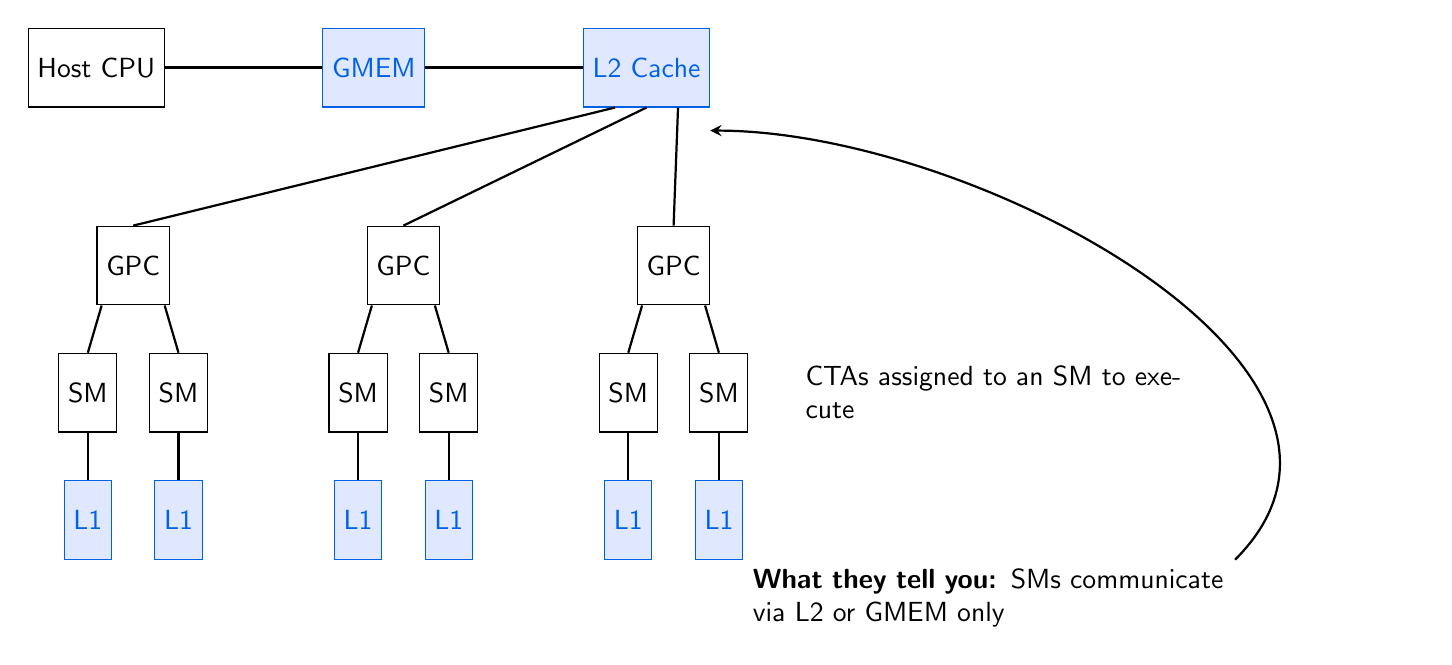
\begin{tikzpicture}[node distance=0mm]

\node (L2) [basic, bluestyle] {L2 Cache};
\node (gmem) [basic, bluestyle, xshift=-20mm, anchor=east] at(L2.west) {GMEM};
\node (cpu) [basic, xshift=-20mm, anchor=east] at(gmem.west) {Host CPU};
\draw [line] (gmem.east) -- (L2.west);
\draw [line] (cpu.east) -- (gmem.west);

\node (gpc2) [basic, anchor=north east, yshift=-15mm] at(L2.south east) {GPC};
\node (gpc1) [basic, anchor=east, xshift=-25mm] at(gpc2.west) {GPC};
\node (gpc0) [basic, anchor=east, xshift=-25mm] at(gpc1.west) {GPC};

\node (sm00) [basic, anchor=north east, yshift=-6mm, xshift=-2mm] at(gpc0.south) {SM};
\node (sm01) [basic, anchor=north west, yshift=-6mm, xshift=+2mm] at(gpc0.south) {SM};
\node (sm10) [basic, anchor=north east, yshift=-6mm, xshift=-2mm] at(gpc1.south) {SM};
\node (sm11) [basic, anchor=north west, yshift=-6mm, xshift=+2mm] at(gpc1.south) {SM};
\node (sm20) [basic, anchor=north east, yshift=-6mm, xshift=-2mm] at(gpc2.south) {SM};
\node (sm21) [basic, anchor=north west, yshift=-6mm, xshift=+2mm] at(gpc2.south) {SM};

\node (L1_00) [basic, bluestyle, anchor=north, yshift=-6mm] at(sm00.south) {L1};
\node (L1_01) [basic, bluestyle, anchor=north, yshift=-6mm] at(sm01.south) {L1};
\node (L1_10) [basic, bluestyle, anchor=north, yshift=-6mm] at(sm10.south) {L1};
\node (L1_11) [basic, bluestyle, anchor=north, yshift=-6mm] at(sm11.south) {L1};
\node (L1_20) [basic, bluestyle, anchor=north, yshift=-6mm] at(sm20.south) {L1};
\node (L1_21) [basic, bluestyle, anchor=north, yshift=-6mm] at(sm21.south) {L1};

\draw [line] ($(gpc0.south) + (-4mm, 0)$) -- (sm00.north);
\draw [line] ($(gpc0.south) + (+4mm, 0)$) -- (sm01.north);
\draw [line] (sm00.south) -- (L1_00.north);
\draw [line] (sm01.south) -- (L1_01.north);
\draw [line] ($(gpc1.south) + (-4mm, 0)$) -- (sm10.north);
\draw [line] ($(gpc1.south) + (+4mm, 0)$) -- (sm11.north);
\draw [line] (sm10.south) -- (L1_10.north);
\draw [line] (sm11.south) -- (L1_11.north);
\draw [line] ($(gpc2.south) + (-4mm, 0)$) -- (sm20.north);
\draw [line] ($(gpc2.south) + (+4mm, 0)$) -- (sm21.north);
\draw [line] (sm20.south) -- (L1_20.north);
\draw [line] (sm21.south) -- (L1_21.north);

\draw [line] ($(L2.south) + (4mm, 0)$) -- (gpc2.north);
\draw [line] ($(L2.south) + (0mm, 0)$) -- (gpc1.north);
\draw [line] ($(L2.south) + (-4mm, 0)$) -- (gpc0.north);

\node(cta) [text width=50mm, anchor=west, xshift=6mm] at(sm21.east) {CTAs assigned to an SM to execute};

\node(note) [text width=60mm, anchor=north west] at(L1_21.south east) {\textbf{What they tell you:} SMs communicate via L2 or GMEM only};

\draw [arrow] (note.north east) to[out=45, in=0] ($(L2.east) + (0, -8mm)$);

\end{tikzpicture}
}
\vfill
Public Sources: \webText{Patent US7564456}{https://patents.google.com/patent/US7564456}, \webText{VR-Pipe: Streamlining Hardware Graphics Pipeline for Volume Rendering}{https://arxiv.org/html/2502.17078v1}


\newpage
\myBiggerTitle{GPU Hardware: Graphics Perspective (Tiling)}

{\large
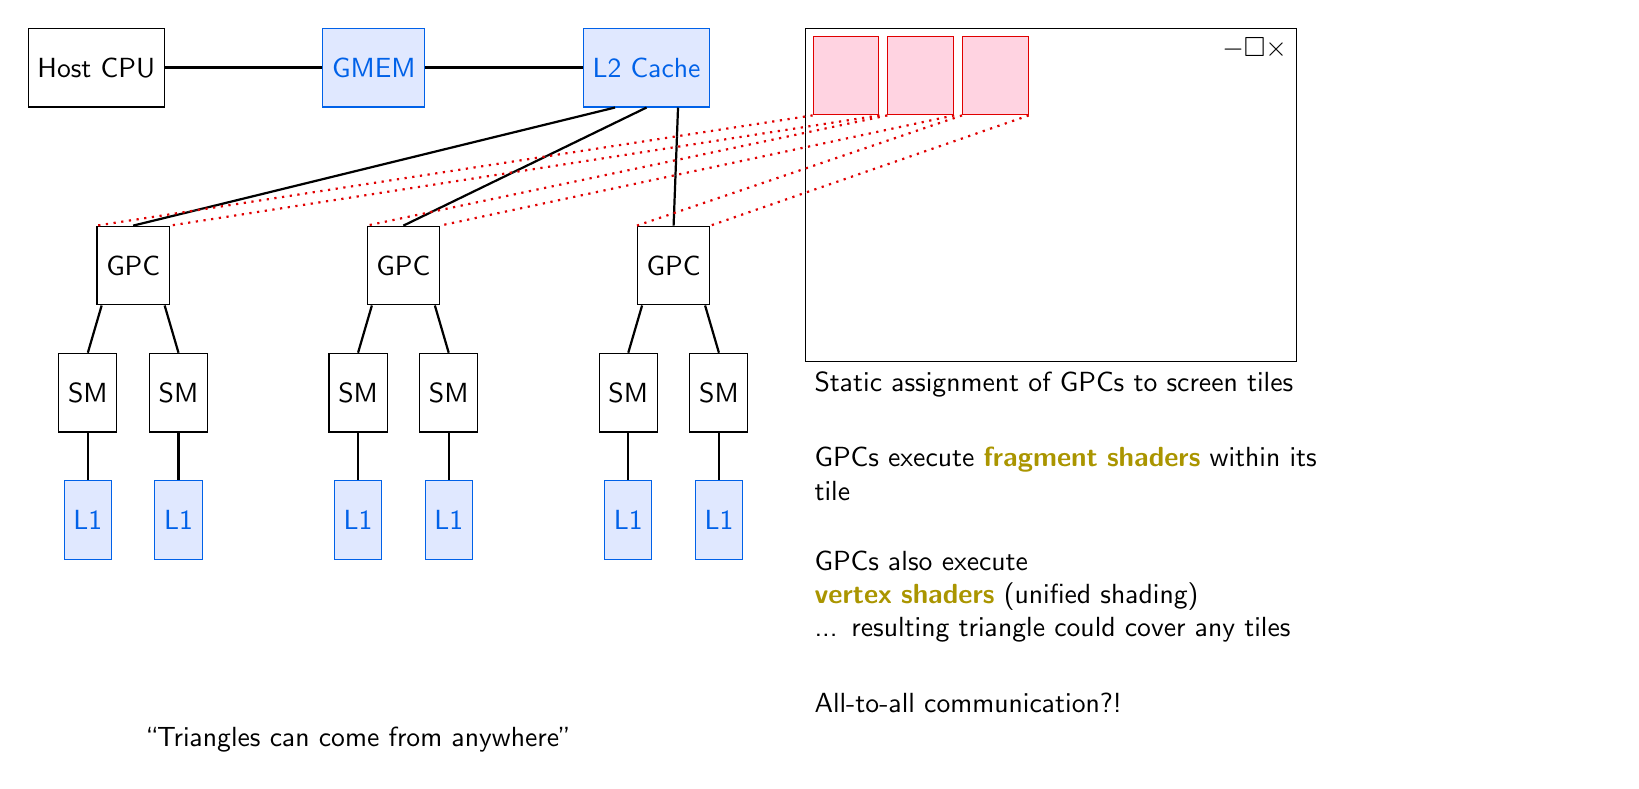
\begin{tikzpicture}[node distance=0mm]

\node (L2) [basic, bluestyle] {L2 Cache};
\node (gmem) [basic, bluestyle, xshift=-20mm, anchor=east] at(L2.west) {GMEM};
\node (cpu) [basic, xshift=-20mm, anchor=east] at(gmem.west) {Host CPU};
\draw [line] (gmem.east) -- (L2.west);
\draw [line] (cpu.east) -- (gmem.west);

\node (gpc2) [basic, anchor=north east, yshift=-15mm] at(L2.south east) {GPC};
\node (gpc1) [basic, anchor=east, xshift=-25mm] at(gpc2.west) {GPC};
\node (gpc0) [basic, anchor=east, xshift=-25mm] at(gpc1.west) {GPC};

\node (sm00) [basic, anchor=north east, yshift=-6mm, xshift=-2mm] at(gpc0.south) {SM};
\node (sm01) [basic, anchor=north west, yshift=-6mm, xshift=+2mm] at(gpc0.south) {SM};
\node (sm10) [basic, anchor=north east, yshift=-6mm, xshift=-2mm] at(gpc1.south) {SM};
\node (sm11) [basic, anchor=north west, yshift=-6mm, xshift=+2mm] at(gpc1.south) {SM};
\node (sm20) [basic, anchor=north east, yshift=-6mm, xshift=-2mm] at(gpc2.south) {SM};
\node (sm21) [basic, anchor=north west, yshift=-6mm, xshift=+2mm] at(gpc2.south) {SM};

\node (L1_00) [basic, bluestyle, anchor=north, yshift=-6mm] at(sm00.south) {L1};
\node (L1_01) [basic, bluestyle, anchor=north, yshift=-6mm] at(sm01.south) {L1};
\node (L1_10) [basic, bluestyle, anchor=north, yshift=-6mm] at(sm10.south) {L1};
\node (L1_11) [basic, bluestyle, anchor=north, yshift=-6mm] at(sm11.south) {L1};
\node (L1_20) [basic, bluestyle, anchor=north, yshift=-6mm] at(sm20.south) {L1};
\node (L1_21) [basic, bluestyle, anchor=north, yshift=-6mm] at(sm21.south) {L1};

\draw [line] ($(gpc0.south) + (-4mm, 0)$) -- (sm00.north);
\draw [line] ($(gpc0.south) + (+4mm, 0)$) -- (sm01.north);
\draw [line] (sm00.south) -- (L1_00.north);
\draw [line] (sm01.south) -- (L1_01.north);
\draw [line] ($(gpc1.south) + (-4mm, 0)$) -- (sm10.north);
\draw [line] ($(gpc1.south) + (+4mm, 0)$) -- (sm11.north);
\draw [line] (sm10.south) -- (L1_10.north);
\draw [line] (sm11.south) -- (L1_11.north);
\draw [line] ($(gpc2.south) + (-4mm, 0)$) -- (sm20.north);
\draw [line] ($(gpc2.south) + (+4mm, 0)$) -- (sm21.north);
\draw [line] (sm20.south) -- (L1_20.north);
\draw [line] (sm21.south) -- (L1_21.north);

\draw [line] ($(L2.south) + (4mm, 0)$) -- (gpc2.north);
\draw [line] ($(L2.south) + (0mm, 0)$) -- (gpc1.north);
\draw [line] ($(L2.south) + (-4mm, 0)$) -- (gpc0.north);
\node(screen) [basic, text width=60mm, text height=40mm, anchor=north west, xshift=12mm] at(L2.north east) {};
\node(controls) [anchor=north east] at(screen.north east) {$-\Box\times$};  % LOL
\node(tile0) [basic, redstyle, text width=6mm, text height=6mm, xshift=1mm, yshift=-1mm, anchor=north west] at(screen.north west) {};
\node(tile1) [basic, redstyle, text width=6mm, text height=6mm, xshift=1mm, anchor=north west] at(tile0.north east) {};
\node(tile2) [basic, redstyle, text width=6mm, text height=6mm, xshift=1mm, anchor=north west] at(tile1.north east) {};

\draw [line, dotted, redstyle] (tile0.south west) -- (gpc0.north west);
\draw [line, dotted, redstyle] (tile0.south east) -- (gpc0.north east);
\draw [line, dotted, redstyle] (tile1.south west) -- (gpc1.north west);
\draw [line, dotted, redstyle] (tile1.south east) -- (gpc1.north east);
\draw [line, dotted, redstyle] (tile2.south west) -- (gpc2.north west);
\draw [line, dotted, redstyle] (tile2.south east) -- (gpc2.north east);


\node(tileNote) [text width=65mm, anchor=north west] at(screen.south west) {Static assignment of GPCs to screen tiles};
\node(fragment) [text width=65mm, anchor=north west, yshift=-4mm] at(tileNote.south west) {GPCs execute \myKeyA{fragment shaders} within its tile};
\node(vertex) [text width=100mm, anchor=north west, yshift=-4mm] at(fragment.south west) {GPCs also execute\\\myKeyA{vertex shaders} (unified shading)\\... resulting triangle could cover any tiles};
\node(allNote) [text width=65mm, anchor=north west, yshift=-4mm] at(vertex.south west) {All-to-all communication?!};

\node(trianglesNote) [anchor=north, yshift=-20mm] at(L1_10.south) {``Triangles can come from anywhere''};

\end{tikzpicture}

}
\vfill
Public Sources: \webText{Patent US7564456}{https://patents.google.com/patent/US7564456}, \webText{VR-Pipe: Streamlining Hardware Graphics Pipeline for Volume Rendering}{https://arxiv.org/html/2502.17078v1}


\newpage
\myBiggerTitle{GPU Hardware: Graphics Perspective (Crossbar)}

{\large
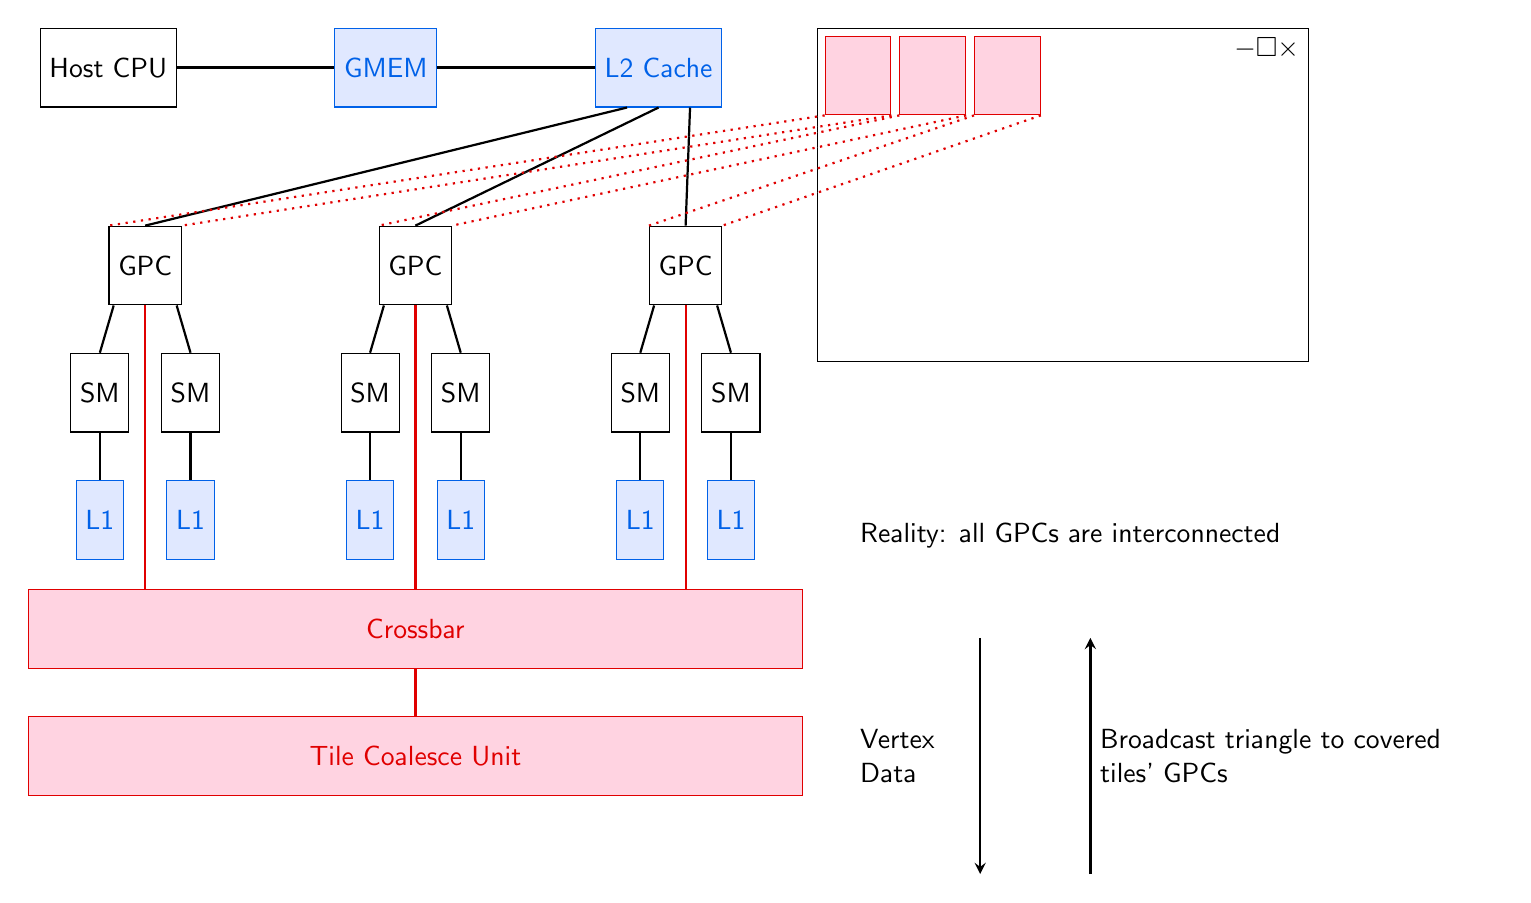
\begin{tikzpicture}[node distance=0mm]

\node (L2) [basic, bluestyle] {L2 Cache};
\node (gmem) [basic, bluestyle, xshift=-20mm, anchor=east] at(L2.west) {GMEM};
\node (cpu) [basic, xshift=-20mm, anchor=east] at(gmem.west) {Host CPU};
\draw [line] (gmem.east) -- (L2.west);
\draw [line] (cpu.east) -- (gmem.west);

\node (gpc2) [basic, anchor=north east, yshift=-15mm] at(L2.south east) {GPC};
\node (gpc1) [basic, anchor=east, xshift=-25mm] at(gpc2.west) {GPC};
\node (gpc0) [basic, anchor=east, xshift=-25mm] at(gpc1.west) {GPC};

\node (sm00) [basic, anchor=north east, yshift=-6mm, xshift=-2mm] at(gpc0.south) {SM};
\node (sm01) [basic, anchor=north west, yshift=-6mm, xshift=+2mm] at(gpc0.south) {SM};
\node (sm10) [basic, anchor=north east, yshift=-6mm, xshift=-2mm] at(gpc1.south) {SM};
\node (sm11) [basic, anchor=north west, yshift=-6mm, xshift=+2mm] at(gpc1.south) {SM};
\node (sm20) [basic, anchor=north east, yshift=-6mm, xshift=-2mm] at(gpc2.south) {SM};
\node (sm21) [basic, anchor=north west, yshift=-6mm, xshift=+2mm] at(gpc2.south) {SM};

\node (L1_00) [basic, bluestyle, anchor=north, yshift=-6mm] at(sm00.south) {L1};
\node (L1_01) [basic, bluestyle, anchor=north, yshift=-6mm] at(sm01.south) {L1};
\node (L1_10) [basic, bluestyle, anchor=north, yshift=-6mm] at(sm10.south) {L1};
\node (L1_11) [basic, bluestyle, anchor=north, yshift=-6mm] at(sm11.south) {L1};
\node (L1_20) [basic, bluestyle, anchor=north, yshift=-6mm] at(sm20.south) {L1};
\node (L1_21) [basic, bluestyle, anchor=north, yshift=-6mm] at(sm21.south) {L1};

\draw [line] ($(gpc0.south) + (-4mm, 0)$) -- (sm00.north);
\draw [line] ($(gpc0.south) + (+4mm, 0)$) -- (sm01.north);
\draw [line] (sm00.south) -- (L1_00.north);
\draw [line] (sm01.south) -- (L1_01.north);
\draw [line] ($(gpc1.south) + (-4mm, 0)$) -- (sm10.north);
\draw [line] ($(gpc1.south) + (+4mm, 0)$) -- (sm11.north);
\draw [line] (sm10.south) -- (L1_10.north);
\draw [line] (sm11.south) -- (L1_11.north);
\draw [line] ($(gpc2.south) + (-4mm, 0)$) -- (sm20.north);
\draw [line] ($(gpc2.south) + (+4mm, 0)$) -- (sm21.north);
\draw [line] (sm20.south) -- (L1_20.north);
\draw [line] (sm21.south) -- (L1_21.north);

\draw [line] ($(L2.south) + (4mm, 0)$) -- (gpc2.north);
\draw [line] ($(L2.south) + (0mm, 0)$) -- (gpc1.north);
\draw [line] ($(L2.south) + (-4mm, 0)$) -- (gpc0.north);
\node(screen) [basic, text width=60mm, text height=40mm, anchor=north west, xshift=12mm] at(L2.north east) {};
\node(controls) [anchor=north east] at(screen.north east) {$-\Box\times$};  % LOL
\node(tile0) [basic, redstyle, text width=6mm, text height=6mm, xshift=1mm, yshift=-1mm, anchor=north west] at(screen.north west) {};
\node(tile1) [basic, redstyle, text width=6mm, text height=6mm, xshift=1mm, anchor=north west] at(tile0.north east) {};
\node(tile2) [basic, redstyle, text width=6mm, text height=6mm, xshift=1mm, anchor=north west] at(tile1.north east) {};

\draw [line, dotted, redstyle] (tile0.south west) -- (gpc0.north west);
\draw [line, dotted, redstyle] (tile0.south east) -- (gpc0.north east);
\draw [line, dotted, redstyle] (tile1.south west) -- (gpc1.north west);
\draw [line, dotted, redstyle] (tile1.south east) -- (gpc1.north east);
\draw [line, dotted, redstyle] (tile2.south west) -- (gpc2.north west);
\draw [line, dotted, redstyle] (tile2.south east) -- (gpc2.north east);

\node (crossbar) [basic, redstyle, text width=96mm, anchor=north, yshift=-36mm] at(gpc1.south) {Crossbar};
\node (tile) [basic, redstyle, text width=96mm, anchor=north, yshift=-6mm] at(crossbar.south) {Tile Coalesce Unit};

\draw [line, redstyle] (gpc0.south) -- ($(gpc0.south) - (0mm, 36mm)$);
\draw [line, redstyle] (gpc1.south) -- ($(gpc1.south) - (0mm, 36mm)$);
\draw [line, redstyle] (gpc2.south) -- ($(gpc2.south) - (0mm, 36mm)$);
\draw [line, redstyle] (crossbar.south) -- (tile.north);



\node(note) [anchor=south west, xshift=6mm, yshift=4mm] at(crossbar.north east) {Reality: all GPCs are interconnected};
\node(vertexDown) [anchor=west, text width=14mm, xshift=6mm] at(tile.east) {Vertex Data};
\node(tileUp) [anchor=west, text width=50mm, xshift=14mm] at(vertexDown.east) {Broadcast triangle to covered tiles' GPCs};
\draw[arrow] ($(vertexDown.east)+(0, 15mm)$) -- ($(vertexDown.east)+(0, -15mm)$);
\draw[arrow] ($(tileUp.west)+(0, -15mm)$) -- ($(tileUp.west)+(0, +15mm)$);


\end{tikzpicture}

}
\vfill
Public Sources: \webText{Patent US7564456}{https://patents.google.com/patent/US7564456}, \webText{VR-Pipe: Streamlining Hardware Graphics Pipeline for Volume Rendering}{https://arxiv.org/html/2502.17078v1}


\newpage
\myBiggerTitle{GPU Hardware: Graphics Perspective (Crossbar)}

{\large
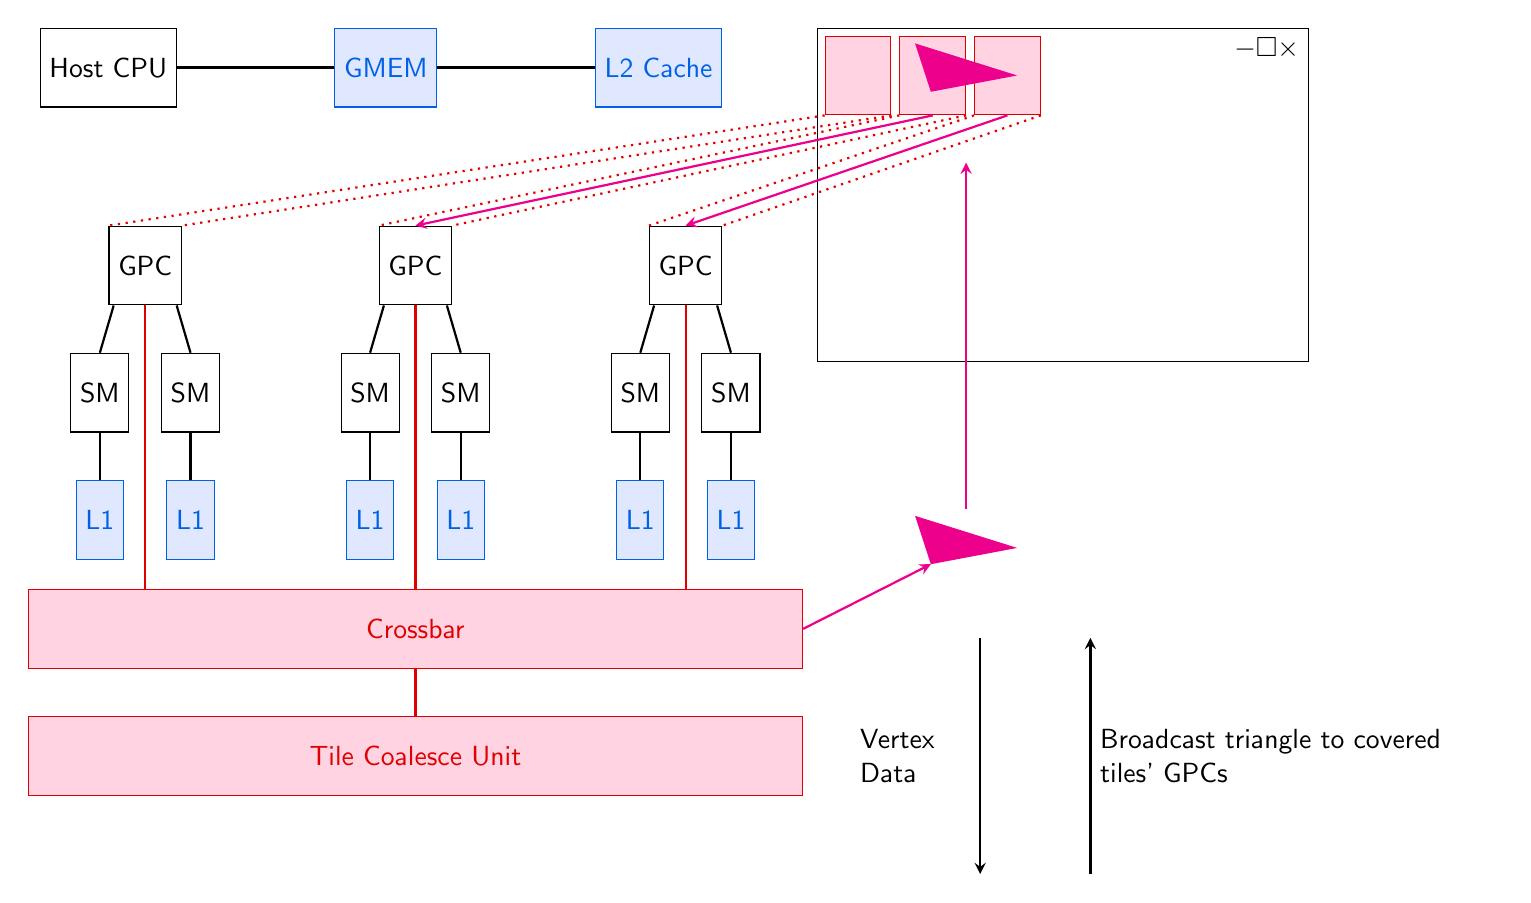
\begin{tikzpicture}[node distance=0mm]

\node (L2) [basic, bluestyle] {L2 Cache};
\node (gmem) [basic, bluestyle, xshift=-20mm, anchor=east] at(L2.west) {GMEM};
\node (cpu) [basic, xshift=-20mm, anchor=east] at(gmem.west) {Host CPU};
\draw [line] (gmem.east) -- (L2.west);
\draw [line] (cpu.east) -- (gmem.west);

\node (gpc2) [basic, anchor=north east, yshift=-15mm] at(L2.south east) {GPC};
\node (gpc1) [basic, anchor=east, xshift=-25mm] at(gpc2.west) {GPC};
\node (gpc0) [basic, anchor=east, xshift=-25mm] at(gpc1.west) {GPC};

\node (sm00) [basic, anchor=north east, yshift=-6mm, xshift=-2mm] at(gpc0.south) {SM};
\node (sm01) [basic, anchor=north west, yshift=-6mm, xshift=+2mm] at(gpc0.south) {SM};
\node (sm10) [basic, anchor=north east, yshift=-6mm, xshift=-2mm] at(gpc1.south) {SM};
\node (sm11) [basic, anchor=north west, yshift=-6mm, xshift=+2mm] at(gpc1.south) {SM};
\node (sm20) [basic, anchor=north east, yshift=-6mm, xshift=-2mm] at(gpc2.south) {SM};
\node (sm21) [basic, anchor=north west, yshift=-6mm, xshift=+2mm] at(gpc2.south) {SM};

\node (L1_00) [basic, bluestyle, anchor=north, yshift=-6mm] at(sm00.south) {L1};
\node (L1_01) [basic, bluestyle, anchor=north, yshift=-6mm] at(sm01.south) {L1};
\node (L1_10) [basic, bluestyle, anchor=north, yshift=-6mm] at(sm10.south) {L1};
\node (L1_11) [basic, bluestyle, anchor=north, yshift=-6mm] at(sm11.south) {L1};
\node (L1_20) [basic, bluestyle, anchor=north, yshift=-6mm] at(sm20.south) {L1};
\node (L1_21) [basic, bluestyle, anchor=north, yshift=-6mm] at(sm21.south) {L1};

\draw [line] ($(gpc0.south) + (-4mm, 0)$) -- (sm00.north);
\draw [line] ($(gpc0.south) + (+4mm, 0)$) -- (sm01.north);
\draw [line] (sm00.south) -- (L1_00.north);
\draw [line] (sm01.south) -- (L1_01.north);
\draw [line] ($(gpc1.south) + (-4mm, 0)$) -- (sm10.north);
\draw [line] ($(gpc1.south) + (+4mm, 0)$) -- (sm11.north);
\draw [line] (sm10.south) -- (L1_10.north);
\draw [line] (sm11.south) -- (L1_11.north);
\draw [line] ($(gpc2.south) + (-4mm, 0)$) -- (sm20.north);
\draw [line] ($(gpc2.south) + (+4mm, 0)$) -- (sm21.north);
\draw [line] (sm20.south) -- (L1_20.north);
\draw [line] (sm21.south) -- (L1_21.north);

\node(screen) [basic, text width=60mm, text height=40mm, anchor=north west, xshift=12mm] at(L2.north east) {};
\node(controls) [anchor=north east] at(screen.north east) {$-\Box\times$};  % LOL
\node(tile0) [basic, redstyle, text width=6mm, text height=6mm, xshift=1mm, yshift=-1mm, anchor=north west] at(screen.north west) {};
\node(tile1) [basic, redstyle, text width=6mm, text height=6mm, xshift=1mm, anchor=north west] at(tile0.north east) {};
\node(tile2) [basic, redstyle, text width=6mm, text height=6mm, xshift=1mm, anchor=north west] at(tile1.north east) {};

\draw [line, dotted, redstyle] (tile0.south west) -- (gpc0.north west);
\draw [line, dotted, redstyle] (tile0.south east) -- (gpc0.north east);
\draw [line, dotted, redstyle] (tile1.south west) -- (gpc1.north west);
\draw [line, dotted, redstyle] (tile1.south east) -- (gpc1.north east);
\draw [line, dotted, redstyle] (tile2.south west) -- (gpc2.north west);
\draw [line, dotted, redstyle] (tile2.south east) -- (gpc2.north east);

\node (crossbar) [basic, redstyle, text width=96mm, anchor=north, yshift=-36mm] at(gpc1.south) {Crossbar};
\node (tile) [basic, redstyle, text width=96mm, anchor=north, yshift=-6mm] at(crossbar.south) {Tile Coalesce Unit};

\draw [line, redstyle] (gpc0.south) -- ($(gpc0.south) - (0mm, 36mm)$);
\draw [line, redstyle] (gpc1.south) -- ($(gpc1.south) - (0mm, 36mm)$);
\draw [line, redstyle] (gpc2.south) -- ($(gpc2.south) - (0mm, 36mm)$);
\draw [line, redstyle] (crossbar.south) -- (tile.north);



\node(vertexDown) [anchor=west, text width=14mm, xshift=6mm] at(tile.east) {Vertex Data};
\node(tileUp) [anchor=west, text width=50mm, xshift=14mm] at(vertexDown.east) {Broadcast triangle to covered tiles' GPCs};
\draw[arrow] ($(vertexDown.east)+(0, 15mm)$) -- ($(vertexDown.east)+(0, -15mm)$);
\draw[arrow] ($(tileUp.west)+(0, -15mm)$) -- ($(tileUp.west)+(0, +15mm)$);


\fill [magenta] ($(tile1.north west)+(2mm, -1mm)$) -- ($(tile1.south west)+(4mm, 3mm)$) -- ($(tile2.east)+(-3mm, 0mm)$) -- cycle;
\fill [magenta] ($(tile1.north west)+(2mm, -61mm)$) -- ($(tile1.south west)+(4mm, -57mm)$) -- ($(tile2.east)+(-3mm, -60mm)$) -- cycle;
\draw [arrow, magenta] (crossbar.east) -- ($(tile1.south west)+(4mm, -57mm)$);
\draw [arrow, magenta] ($(tile1.south east)+(0mm, -50mm)$) -- ($(tile1.south east)+(0mm, -6mm)$);
\draw [arrow, magenta] (tile1.south) -- (gpc1.north);
\draw [arrow, magenta] (tile2.south) -- (gpc2.north);

\end{tikzpicture}

}
\vfill
Public Sources: \webText{Patent US7564456}{https://patents.google.com/patent/US7564456}, \webText{VR-Pipe: Streamlining Hardware Graphics Pipeline for Volume Rendering}{https://arxiv.org/html/2502.17078v1}


\newpage
\myBiggerTitle{GPU Hardware: Graphics Perspective (ROPs)}

{\large
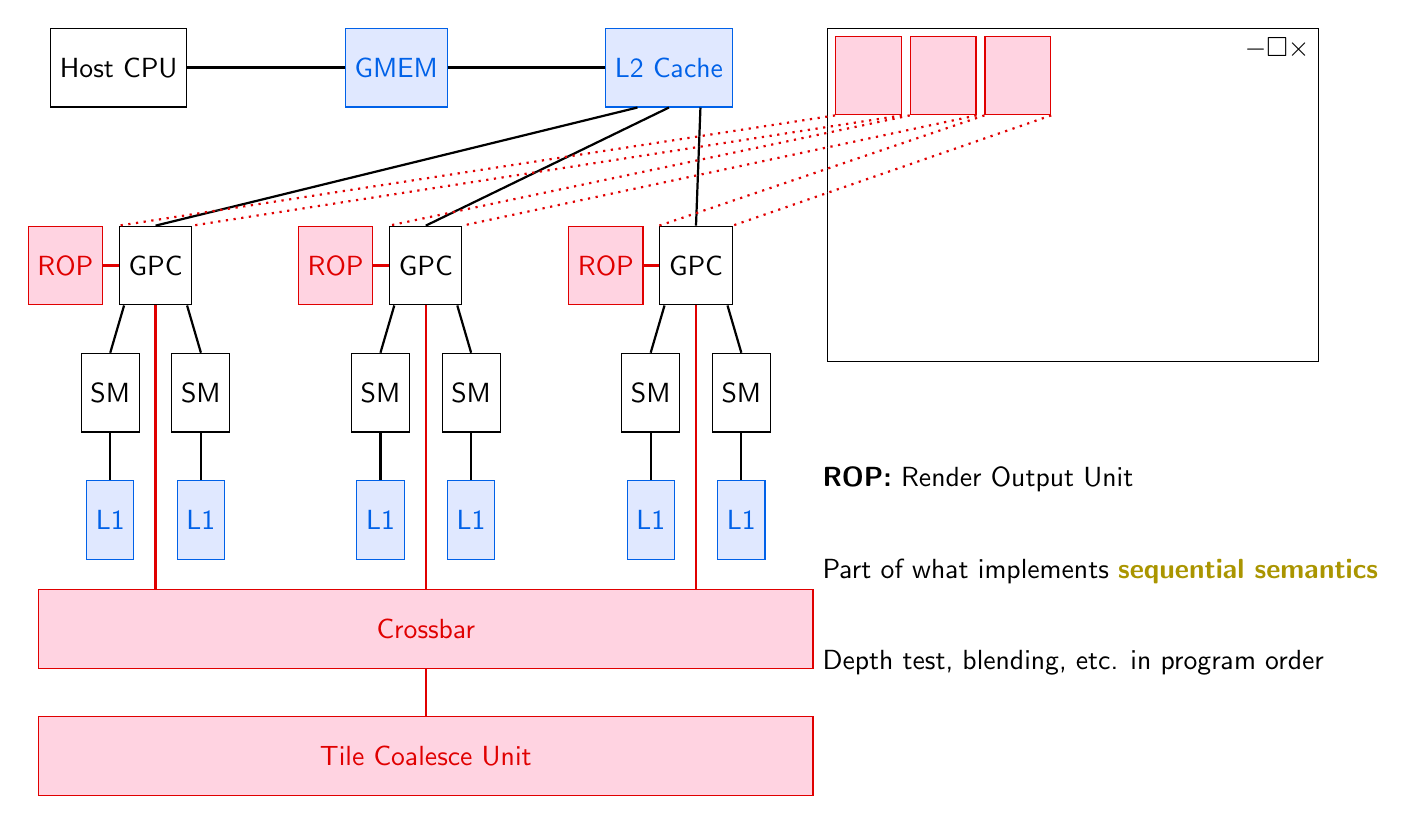
\begin{tikzpicture}[node distance=0mm]

\node (L2) [basic, bluestyle] {L2 Cache};
\node (gmem) [basic, bluestyle, xshift=-20mm, anchor=east] at(L2.west) {GMEM};
\node (cpu) [basic, xshift=-20mm, anchor=east] at(gmem.west) {Host CPU};
\draw [line] (gmem.east) -- (L2.west);
\draw [line] (cpu.east) -- (gmem.west);

\node (gpc2) [basic, anchor=north east, yshift=-15mm] at(L2.south east) {GPC};
\node (gpc1) [basic, anchor=east, xshift=-25mm] at(gpc2.west) {GPC};
\node (gpc0) [basic, anchor=east, xshift=-25mm] at(gpc1.west) {GPC};

\node (sm00) [basic, anchor=north east, yshift=-6mm, xshift=-2mm] at(gpc0.south) {SM};
\node (sm01) [basic, anchor=north west, yshift=-6mm, xshift=+2mm] at(gpc0.south) {SM};
\node (sm10) [basic, anchor=north east, yshift=-6mm, xshift=-2mm] at(gpc1.south) {SM};
\node (sm11) [basic, anchor=north west, yshift=-6mm, xshift=+2mm] at(gpc1.south) {SM};
\node (sm20) [basic, anchor=north east, yshift=-6mm, xshift=-2mm] at(gpc2.south) {SM};
\node (sm21) [basic, anchor=north west, yshift=-6mm, xshift=+2mm] at(gpc2.south) {SM};

\node (L1_00) [basic, bluestyle, anchor=north, yshift=-6mm] at(sm00.south) {L1};
\node (L1_01) [basic, bluestyle, anchor=north, yshift=-6mm] at(sm01.south) {L1};
\node (L1_10) [basic, bluestyle, anchor=north, yshift=-6mm] at(sm10.south) {L1};
\node (L1_11) [basic, bluestyle, anchor=north, yshift=-6mm] at(sm11.south) {L1};
\node (L1_20) [basic, bluestyle, anchor=north, yshift=-6mm] at(sm20.south) {L1};
\node (L1_21) [basic, bluestyle, anchor=north, yshift=-6mm] at(sm21.south) {L1};

\draw [line] ($(gpc0.south) + (-4mm, 0)$) -- (sm00.north);
\draw [line] ($(gpc0.south) + (+4mm, 0)$) -- (sm01.north);
\draw [line] (sm00.south) -- (L1_00.north);
\draw [line] (sm01.south) -- (L1_01.north);
\draw [line] ($(gpc1.south) + (-4mm, 0)$) -- (sm10.north);
\draw [line] ($(gpc1.south) + (+4mm, 0)$) -- (sm11.north);
\draw [line] (sm10.south) -- (L1_10.north);
\draw [line] (sm11.south) -- (L1_11.north);
\draw [line] ($(gpc2.south) + (-4mm, 0)$) -- (sm20.north);
\draw [line] ($(gpc2.south) + (+4mm, 0)$) -- (sm21.north);
\draw [line] (sm20.south) -- (L1_20.north);
\draw [line] (sm21.south) -- (L1_21.north);

\draw [line] ($(L2.south) + (4mm, 0)$) -- (gpc2.north);
\draw [line] ($(L2.south) + (0mm, 0)$) -- (gpc1.north);
\draw [line] ($(L2.south) + (-4mm, 0)$) -- (gpc0.north);
\node (crossbar) [basic, redstyle, text width=96mm, anchor=north, yshift=-36mm] at(gpc1.south) {Crossbar};
\node (tile) [basic, redstyle, text width=96mm, anchor=north, yshift=-6mm] at(crossbar.south) {Tile Coalesce Unit};

\draw [line, redstyle] (gpc0.south) -- ($(gpc0.south) - (0mm, 36mm)$);
\draw [line, redstyle] (gpc1.south) -- ($(gpc1.south) - (0mm, 36mm)$);
\draw [line, redstyle] (gpc2.south) -- ($(gpc2.south) - (0mm, 36mm)$);
\draw [line, redstyle] (crossbar.south) -- (tile.north);


\node(screen) [basic, text width=60mm, text height=40mm, anchor=north west, xshift=12mm] at(L2.north east) {};
\node(controls) [anchor=north east] at(screen.north east) {$-\Box\times$};  % LOL
\node(tile0) [basic, redstyle, text width=6mm, text height=6mm, xshift=1mm, yshift=-1mm, anchor=north west] at(screen.north west) {};
\node(tile1) [basic, redstyle, text width=6mm, text height=6mm, xshift=1mm, anchor=north west] at(tile0.north east) {};
\node(tile2) [basic, redstyle, text width=6mm, text height=6mm, xshift=1mm, anchor=north west] at(tile1.north east) {};

\draw [line, dotted, redstyle] (tile0.south west) -- (gpc0.north west);
\draw [line, dotted, redstyle] (tile0.south east) -- (gpc0.north east);
\draw [line, dotted, redstyle] (tile1.south west) -- (gpc1.north west);
\draw [line, dotted, redstyle] (tile1.south east) -- (gpc1.north east);
\draw [line, dotted, redstyle] (tile2.south west) -- (gpc2.north west);
\draw [line, dotted, redstyle] (tile2.south east) -- (gpc2.north east);

\node (rop0) [basic, redstyle, anchor=east, xshift=-2mm] at(gpc0.west) {ROP};
\node (rop1) [basic, redstyle, anchor=east, xshift=-2mm] at(gpc1.west) {ROP};
\node (rop2) [basic, redstyle, anchor=east, xshift=-2mm] at(gpc2.west) {ROP};
\draw [line, redstyle] (rop0.east) -- (gpc0.west);
\draw [line, redstyle] (rop1.east) -- (gpc1.west);
\draw [line, redstyle] (rop2.east) -- (gpc2.west);


\node (ropNote) [anchor=west, xshift=+6mm] at(L1_21.north east) {\textbf{ROP:} Render Output Unit};

\node (seqNote) [anchor=north west, yshift=-6mm] at(ropNote.south west) {Part of what implements \myKeyA{sequential semantics}};

\node [anchor=north west, yshift=-6mm] at(seqNote.south west) {Depth test, blending, etc. in program order};

\end{tikzpicture}

}
\vfill
Public Sources: \webText{Patent US7564456}{https://patents.google.com/patent/US7564456}, \webText{VR-Pipe: Streamlining Hardware Graphics Pipeline for Volume Rendering}{https://arxiv.org/html/2502.17078v1}


\newpage

\begin{minipage}[t]{0.68\textwidth}\fixminipage
{\myBiggerTitle{Myricube: Chunks}

\LARGE

Divide world into $16 \times 16 \times 16$ \emph{chunks}
\begin{itemize}
  \item Stores raw array of voxels
\end{itemize}

\vspace{4mm}

Compute AABB (axis-aligned bounding box) of opaque voxels in the chunk

\vspace{4mm}

Draw AABB (12 triangles), \myKeyA{fragment shader} raycasts based on voxels in chunk

\vspace{4mm}

\myKeyA{Discard} if no voxel hit

}
\end{minipage}
\hfill
\begin{minipage}[t]{0.3\textwidth}\fixminipage
\hphantom{Hello}
\includegraphics[width=\linewidth] {myricube/many_chunks_0.jpg}

\includegraphics[width=\linewidth] {myricube/many_chunks_1.jpg}
\end{minipage}

\newpage
\includegraphics[width=\linewidth] {myricube/myricube_chunk_flow_0.jpg}
\newpage
\includegraphics[width=\linewidth] {myricube/myricube_chunk_flow_1.jpg}
\newpage
\includegraphics[width=\linewidth] {myricube/myricube_chunk_flow_2.jpg}
\newpage
\includegraphics[width=\linewidth] {myricube/myricube_chunk_flow_3.jpg}
\newpage
\includegraphics[width=\linewidth] {myricube/myricube_chunk_flow_0.jpg}

\newpage
\myBiggerTitle{Demo 1}

{\LARGE
\hfill(we'll do it live)

}

\newpage
\myBiggerTitle{Early z-culling}

{\LARGE

Issue: what about chunks that are hidden behind something else?
\begin{itemize}
  \item Depth testing ensures front-most chunk ``wins''
  \item ... but are we wasting time drawing hidden chunks?
\end{itemize}
\vspace{8mm}
Should we do occlusion culling?

}

\newpage
\myBiggerTitle{Early z-culling: Hardware}

{\large
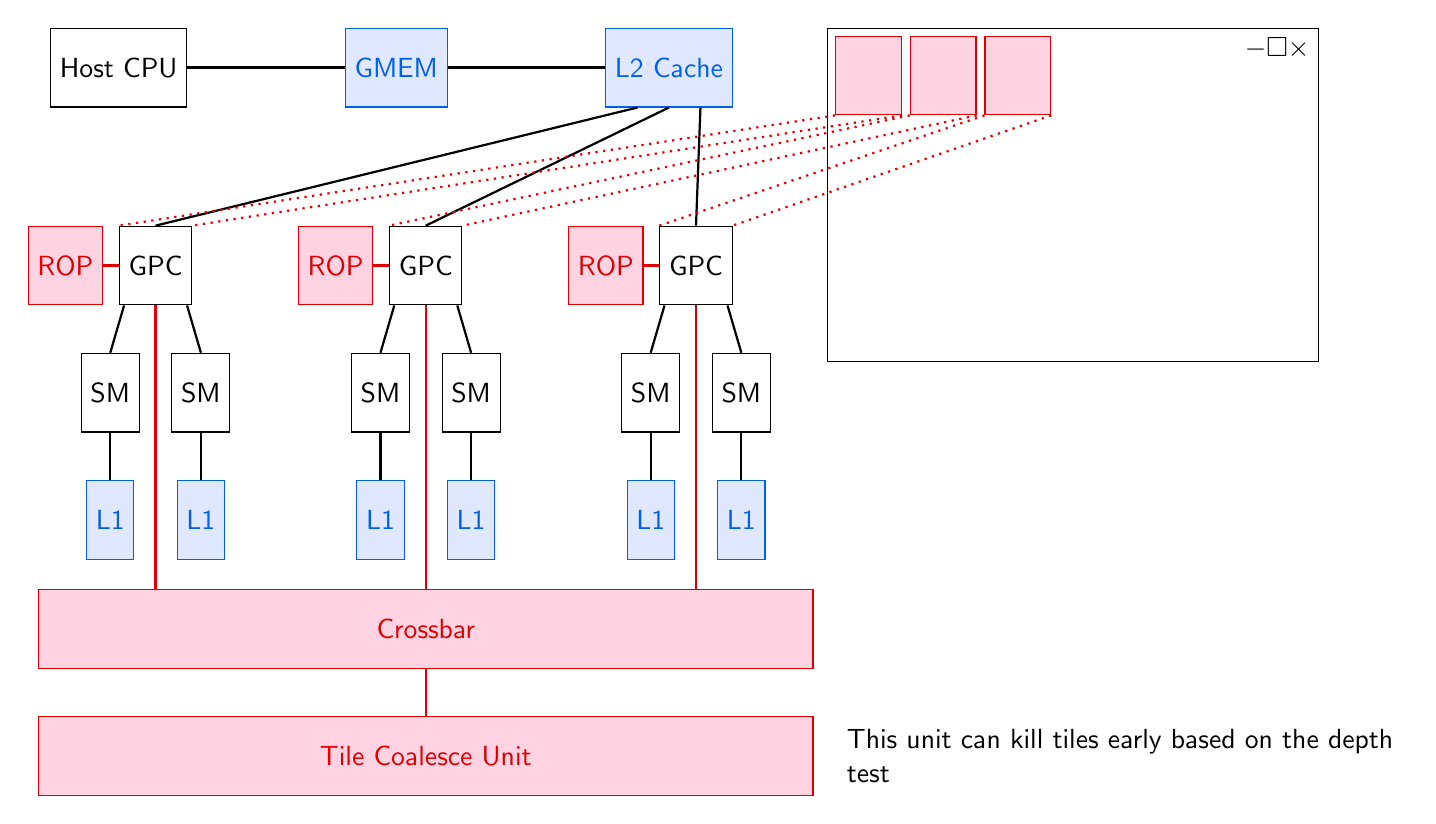
\begin{tikzpicture}[node distance=0mm]

\node (L2) [basic, bluestyle] {L2 Cache};
\node (gmem) [basic, bluestyle, xshift=-20mm, anchor=east] at(L2.west) {GMEM};
\node (cpu) [basic, xshift=-20mm, anchor=east] at(gmem.west) {Host CPU};
\draw [line] (gmem.east) -- (L2.west);
\draw [line] (cpu.east) -- (gmem.west);

\node (gpc2) [basic, anchor=north east, yshift=-15mm] at(L2.south east) {GPC};
\node (gpc1) [basic, anchor=east, xshift=-25mm] at(gpc2.west) {GPC};
\node (gpc0) [basic, anchor=east, xshift=-25mm] at(gpc1.west) {GPC};

\node (sm00) [basic, anchor=north east, yshift=-6mm, xshift=-2mm] at(gpc0.south) {SM};
\node (sm01) [basic, anchor=north west, yshift=-6mm, xshift=+2mm] at(gpc0.south) {SM};
\node (sm10) [basic, anchor=north east, yshift=-6mm, xshift=-2mm] at(gpc1.south) {SM};
\node (sm11) [basic, anchor=north west, yshift=-6mm, xshift=+2mm] at(gpc1.south) {SM};
\node (sm20) [basic, anchor=north east, yshift=-6mm, xshift=-2mm] at(gpc2.south) {SM};
\node (sm21) [basic, anchor=north west, yshift=-6mm, xshift=+2mm] at(gpc2.south) {SM};

\node (L1_00) [basic, bluestyle, anchor=north, yshift=-6mm] at(sm00.south) {L1};
\node (L1_01) [basic, bluestyle, anchor=north, yshift=-6mm] at(sm01.south) {L1};
\node (L1_10) [basic, bluestyle, anchor=north, yshift=-6mm] at(sm10.south) {L1};
\node (L1_11) [basic, bluestyle, anchor=north, yshift=-6mm] at(sm11.south) {L1};
\node (L1_20) [basic, bluestyle, anchor=north, yshift=-6mm] at(sm20.south) {L1};
\node (L1_21) [basic, bluestyle, anchor=north, yshift=-6mm] at(sm21.south) {L1};

\draw [line] ($(gpc0.south) + (-4mm, 0)$) -- (sm00.north);
\draw [line] ($(gpc0.south) + (+4mm, 0)$) -- (sm01.north);
\draw [line] (sm00.south) -- (L1_00.north);
\draw [line] (sm01.south) -- (L1_01.north);
\draw [line] ($(gpc1.south) + (-4mm, 0)$) -- (sm10.north);
\draw [line] ($(gpc1.south) + (+4mm, 0)$) -- (sm11.north);
\draw [line] (sm10.south) -- (L1_10.north);
\draw [line] (sm11.south) -- (L1_11.north);
\draw [line] ($(gpc2.south) + (-4mm, 0)$) -- (sm20.north);
\draw [line] ($(gpc2.south) + (+4mm, 0)$) -- (sm21.north);
\draw [line] (sm20.south) -- (L1_20.north);
\draw [line] (sm21.south) -- (L1_21.north);

\draw [line] ($(L2.south) + (4mm, 0)$) -- (gpc2.north);
\draw [line] ($(L2.south) + (0mm, 0)$) -- (gpc1.north);
\draw [line] ($(L2.south) + (-4mm, 0)$) -- (gpc0.north);
\node (crossbar) [basic, redstyle, text width=96mm, anchor=north, yshift=-36mm] at(gpc1.south) {Crossbar};
\node (tile) [basic, redstyle, text width=96mm, anchor=north, yshift=-6mm] at(crossbar.south) {Tile Coalesce Unit};

\draw [line, redstyle] (gpc0.south) -- ($(gpc0.south) - (0mm, 36mm)$);
\draw [line, redstyle] (gpc1.south) -- ($(gpc1.south) - (0mm, 36mm)$);
\draw [line, redstyle] (gpc2.south) -- ($(gpc2.south) - (0mm, 36mm)$);
\draw [line, redstyle] (crossbar.south) -- (tile.north);


\node(screen) [basic, text width=60mm, text height=40mm, anchor=north west, xshift=12mm] at(L2.north east) {};
\node(controls) [anchor=north east] at(screen.north east) {$-\Box\times$};  % LOL
\node(tile0) [basic, redstyle, text width=6mm, text height=6mm, xshift=1mm, yshift=-1mm, anchor=north west] at(screen.north west) {};
\node(tile1) [basic, redstyle, text width=6mm, text height=6mm, xshift=1mm, anchor=north west] at(tile0.north east) {};
\node(tile2) [basic, redstyle, text width=6mm, text height=6mm, xshift=1mm, anchor=north west] at(tile1.north east) {};

\draw [line, dotted, redstyle] (tile0.south west) -- (gpc0.north west);
\draw [line, dotted, redstyle] (tile0.south east) -- (gpc0.north east);
\draw [line, dotted, redstyle] (tile1.south west) -- (gpc1.north west);
\draw [line, dotted, redstyle] (tile1.south east) -- (gpc1.north east);
\draw [line, dotted, redstyle] (tile2.south west) -- (gpc2.north west);
\draw [line, dotted, redstyle] (tile2.south east) -- (gpc2.north east);

\node (rop0) [basic, redstyle, anchor=east, xshift=-2mm] at(gpc0.west) {ROP};
\node (rop1) [basic, redstyle, anchor=east, xshift=-2mm] at(gpc1.west) {ROP};
\node (rop2) [basic, redstyle, anchor=east, xshift=-2mm] at(gpc2.west) {ROP};
\draw [line, redstyle] (rop0.east) -- (gpc0.west);
\draw [line, redstyle] (rop1.east) -- (gpc1.west);
\draw [line, redstyle] (rop2.east) -- (gpc2.west);


\node [xshift=+3mm, anchor=west, text width=70mm] at(tile.east) {This unit can kill tiles early based on the depth test};

\end{tikzpicture}
}

\vfill
Public Sources: \webText{Patent US7564456}{https://patents.google.com/patent/US7564456}, \webText{VR-Pipe: Streamlining Hardware Graphics Pipeline for Volume Rendering}{https://arxiv.org/html/2502.17078v1}


\newpage
\myBiggerTitle{Early z-culling: Fragment Shading}

{\large
\begin{tikzpicture}[node distance=0mm]

\node(for) [text width=70mm] {For each triangle \myKeyA{in order},\\for each pixel covered\\by the triangle,};

\node(screen) [basic, text width=60mm, text height=40mm, anchor=west] at(for.east) {};
\node(controls) [anchor=north east] at(screen.north east) {$-\Box\times$};  % LOL
\node(dv0) [fill=gray, cheesyvertex, anchor=center, xshift=10mm, yshift=-10mm] at(screen.north west) {};
\node(dv1) [fill=gray, cheesyvertex, anchor=center, xshift=18mm, yshift=-34mm] at(screen.north west) {};
\node(dv2) [fill=gray, cheesyvertex, anchor=center, xshift=50mm, yshift=-13mm] at(screen.north west) {};
\node(dPixel) [fill=black, cheesyvertex, anchor=center, xshift=20mm, yshift=-22mm] at(screen.north west) {};
\draw [dotted] (dv0) -- (dv1);
\draw [dotted] (dv0) -- (dv2);
\draw [dotted] (dv1) -- (dv2);

\node(dColor) [anchor=north east] at(screen.south east) {\textbf{Dest. Color}};
\node(dDepth) [anchor=north east] at(dColor.south east) {\textbf{Dest. Depth}};
\node(sColor) [anchor=north east] at(dDepth.south east) {\textbf{Src. Color}};
\node(sDepth) [anchor=north east] at(sColor.south east) {\textbf{Src. Depth}};

\node(write) [basic, text width=25mm, minimum height=25mm, anchor=west, xshift=45mm] at(dPixel.east) {Write back\\new color,\\new depth};
\draw [arrow] (write.west) -- (dPixel.east);
\node(OR) [anchor=west] at(write.east) {\textbf{OR}};
\node(discard) [basic, text width=25mm, minimum height=25mm, anchor=west] at(OR.east) {\myKeyA{DISCARD}};

\node(sv0) [fill=nRedBoxBg, cheesyvertex, anchor=center, yshift=-75mm] at(dv0.center) {};
\node(sv1) [fill=nGoldBoxBg, cheesyvertex, anchor=center, yshift=-75mm] at(dv1.center) {};
\node(sv2) [fill=nGreenBoxBg, cheesyvertex, anchor=center, yshift=-75mm] at(dv2.center) {};
\node(vs) [anchor=east, xshift=-4mm, yshift=2mm] at(sv1.west) {(from vertex shaders)};
\node(sPixel) [fill=black, cheesyvertex, anchor=center, yshift=-75mm] at(dPixel.center) {};
\draw [dotted] (sv0) -- (sv1);
\draw [dotted] (sv0) -- (sv2);
\draw [dotted] (sv1) -- (sv2);

\node(blending) [basic, anchor=north, yshift=-25mm] at(OR.south) {Blending};
\draw [arrow] (blending) -- ($(OR)+(0, -9mm)$);
\node(depthTest) [basic, text width=40mm, anchor=north west, yshift=-8mm] at(blending.south west) {Depth Test\\\myKeyA{MAY DISCARD}};

\draw [arrow] (dColor.east) to[out=0, in=180] ($(blending.west)+(0, 2mm)$);
\draw [arrow] (sColor.east) to[out=0, in=180] ($(blending.west)+(0, -2mm)$);
\draw [arrow, draw=magenta] (dDepth.east) to[out=0, in=180] ($(depthTest.west)+(0, 2mm)$);
\draw [arrow, draw=magenta] (sDepth.east) to[out=0, in=180] ($(depthTest.west)+(0, -2mm)$);
\draw [arrow] ($(dPixel.south)+(1mm, 0)$) to[out=270, in=180] (dColor.west);
\draw [arrow, draw=magenta] ($(dPixel.south)+(-1mm, 0)$) to[out=270, in=180] (dDepth.west);

\node(fragment) [basic, text width=40mm, anchor=east, xshift=-6mm] at($(sColor.west)!0.5!(sDepth.west)$) {Fragment Shader\\\myKeyA{MAY DISCARD}};
\node(fragmentText) [anchor=north west] at(fragment.south west) {\textbf{1 fragment = 1 thread}};
\node(iDepth) [anchor=east, xshift=-66mm] at(sDepth.west) {\textbf{Interpolated Depth}};
\node(uniforms) [anchor=south, yshift=6mm] at(iDepth.north) {\textbf{Uniforms from CPU}};
\node(iAttrs) [anchor=north, yshift=-6mm, text width=50mm] at(iDepth.south) {\textbf{Interpolated Output\\Vertex Attributes}};

\draw [arrow] ($(fragment.east)+(0, +4mm)$) to[out=0, in=180] (sColor.west);
\draw [arrow, draw=magenta] ($(fragment.east)+(0, -4mm)$) to[out=0, in=180] (sDepth.west);
\draw [arrow, draw=magenta] (iDepth.east) to[out=0, in=180] ($(fragment.west)+(0, -4mm)$);
\draw [arrow] (uniforms.east) to[out=0, in=180] ($(fragment.west)+(0, +4mm)$);
\draw [arrow] (iAttrs.east) to[out=0, in=225] (fragment.south west);
\draw [arrow, draw=magenta] ($(sPixel.west)+(0, 1mm)$) to[out=180, in=315] (iDepth.south east);
\draw [arrow] ($(sPixel.west)+(0, -1mm)$) to[out=180, in=315] (iAttrs.south east);

\node (depthInfo) [text width=75mm, anchor=north east] at(depthTest.south east) {{\color{magenta}\textbf{Depth Idea:}}
Per-pixel depth encodes ``distance from camera'';\\closest fragment wins depth test.};


\node (note1) [redstyle, anchor=east, text width=60mm, xshift=-2mm] at(screen.south west) {Suppose fragment shader has no side effects, \textbf{passes through} depth};
\draw [line, redstyle] (iDepth.north) -- (note1);
\draw [line, redstyle] (sDepth.north) -- (note1);
\node (note2) [redstyle, anchor=north west, text width=80mm, yshift=-4mm] at(depthInfo.north west) {We can skip tiles of fragment shaders if we know they will fail the depth test anyway.};

\end{tikzpicture}
}

\newpage
\myBiggerTitle{Myricube: Reverse Painter's}

{\LARGE

Myricube draws chunks in near-to-far order

Farther chunks \emph{might} be subject to early z-culling
\begin{itemize}
  \item Rely on implicit hardware culling, instead of DIY
\end{itemize}

\vspace{6mm}

Why did the triangle mesh approach need occlusion culling more?

\begin{itemize}
  \item Early-z skips fragment shaders, not vertex shaders
  \item Have to rasterize triangles to know the tiles covered
  \item We only waste 12 triangles (AABB) if we don't cull
  \item Other approach wastes thousands/millions of triangles
\end{itemize}

}

\newpage
\myBiggerTitle{Myricube: Uploads from Disk}

{\LARGE
Chunk Storage:
\begin{itemize}
  \item On CPU: in mmap'd binary files (3D arrays)
  \item On GPU: in 3D texture
  \item Both organized into \myKeyA{chunk groups}, with version number
\end{itemize}
\vspace{4mm}
Background threads listen for CPU/GPU version number mismatches; upon detection, the thread
\begin{itemize}
\item Uses the DMA engine (Vulkan transfer queue) to copy raw voxels from file to 3D texture (faaast)
\item Calculates the new AABB (faaast)
\end{itemize}
\vspace{4mm}
Supports Linux and Windows (pain)

}

\newpage
\myBiggerTitle{Myricube: Uploads from Disk}

{\LARGE
Only copy outdated chunk groups in the camera frustum

Copy-to-GPU finishes asynchronously

Not finished in time?
\begin{itemize}
  \item Draw outdated GPU 3D texture, or skip chunks
\end{itemize}

\vfill

\includegraphics[width=0.333\linewidth]{myricube/myricraft_loading_1.jpg}
\includegraphics[width=0.333\linewidth]{myricube/myricraft_loading_2.jpg}
\includegraphics[width=0.333\linewidth]{myricube/myricraft_loading_3.jpg}

}

\newpage
\myBiggerTitle{Demo 2}

{\LARGE
\hfill(we'll do it live)

}

\newpage
\myBiggerTitle{Questions?} \hfill Planet model by my friend, Marlon Trifunovic

\includegraphics[width=0.495\linewidth]{myricube/marlo_planet_chunks.jpg}
\includegraphics[width=0.495\linewidth]{myricube/marlo_planet.jpg}

\end{document}
